\section{Analysis} \label{sec:analysis}


% Pacman content research


\subsection{Pacman}
\subsubsection{AI behaviour argumentation (how they do it)}
\subsubsection{Technical details/mechanics/paramters}

\subsection{Player performance}
a. Identify pacman parameters to measure player performance. (from 4.B) Associate also with  previous research(other AI implementations in Pacman. What did they use to  identify “performance”?


b. Define “good” and “bad” performance based upon 5a. (assume that we use only win/lose conditions unless prior research has based performance indications upon other game parameter results)

c. Performance results. We identify “some” performance. Therefore we configure the following “alternation of ghost behavior” in “this” way.

\subsection{Genetic Algorithm(s)}

\subsubsection{Description}
Genetic algorithms was invented by John Holland in 1975 and is proposed as a heuristic method, which is a method to learn by itself based upon survival of the fittest, where it is described as a  search algorithm that uses mechanisms much like evolution to improve some solutions to a given problem. \cite[pp. 20]{Sivanandam2008}

The Genetic Algorithm start with a set of plausible solutions and by the use of genetic operator alterations like reproduction, crossovers and mutations \cite{Baltzer2014}, it develops a new set of better solutions compared to the previous. By repeating this process, a population will theoretically improve until a satisfying result is found to the given problem. \cite{BCS2013}

What is noteworthy about "satisfying results" is that we search for some better solution within a set of possible solutions, also referred to as search space. It is therefore not guaranteed to find some, if any, optimal solution to the problem but rather a solution which can be interpreted as acceptably good. \cite[pp. 20/21]{Sivanandam2008}


In genetic algorithms, populations and individuals covers the terminology of the solutions and searches thereof. A individual is to be considered a single solution to the problem and the population is the number of individuals involved. \cite[pp. 39]{Sivanandam2008} 



\subsubsection{Genetic Algorithm Components}

A Genetic Algorithm consists of at least five components as described by Baltzer, 2014 \cite{Baltzer2014}. These components can be considered to be the main components in any genetic algorithm.
\begin{itemize}
\item \textbf{Chromosome / gene representation}

A representation of a population and the subordinate content, being chromosomes and genes as seen on figure \ref{fig:gene}.
The genes functions as a string of some arbitrary length of data. A chromosome is a sequence of genes, whereof the combined chromosomes serves as the population. \cite[pp. 41]{Sivanandam2008} 

As mentioned above, each individual(chromosome) is a single solution to the problem at hand. The chromosomes can be considered to be \enquote{a point in the search space of candidate solutions} \cite[pp. 7]{Melanie1990} Melanie, 1990.
	

\begin{figure}[!h]
\centering
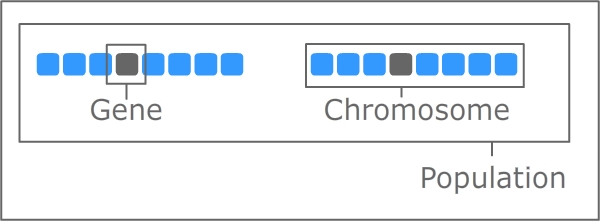
\includegraphics[scale=1.0]{gene_chromosomes.jpg}
\caption{gene, chromosomes and population description}
\label{fig:gene}
\end{figure}

\item \textbf{Initialisation of the population}

A population is a collection of individuals(chromosomes).  

An initial population must be created as a starting point for the algorithm. This representation of a population is chosen randomly, as there might be no prior evident solutions. Dependent on the stated problem at hand, the initialization of populations might also be carried out with some good solutions to the problem. However in most cases, the initial population is chosen at random. \cite[pp. 41/42]{Sivanandam2008}



\item \textbf{evaluation function(fitness)}

In order to improve further generations, the fitness of each chromosome in the current population must be evaluated. The genetic algorithm does so by the use of a fitness function, which assign some score(fitness) to each of the chromosomes within a specific population.
In general manners, the fitness of a given chromosome is dependant on how successively the given chromosome solved the designated problem, and is conveyed through a range of values. The better the solution, the higher the fitness score \cite[pp. 8]{Melanie1990}

how "good" the solution is, is the whole purpose of the fitness function to identify. the fitness function perform some evaluation of the acquired results and then assigns specific fitness score to that solution. How the fitness function performs the evaluation of solution is dependent on the problem itself. There are no single solutions as to how the fitness function is to be developed, but can be really be anything, that successively covers the plausible methods of evaluating the solutions. \cite[pp. 31]{Sivanandam2008}




\item \textbf{Genetic operators altering chromosomes(reproduction/selection, crossover and mutation.}


Genetic operators in some of the more simple Genetic Algorithms are reproduction/selection, crossover and mutation. Melanie, 1990. \cite{Melanie1990}

\textbf{reproduction/selection:} \enquote{This operator selects chromosomes in the population for reproduction. The fitter the chromosome, the more times it is likely to be selected to reproduce.} \cite[pp. 8]{Melanie1990}
The idea behind this operator is that preferences are given to the better chromosomes in the population, which is then passed on to the next generation. This is based upon the fitness score.

Within the selection operator, several selection methods exists which defines how the actual selection of "best" individuals is to be conducted. 

Some of the selection methods are:
\begin{itemize}
\item Roulette Wheel Selection
\item Random Selection
\item Rank Selection
\item Tournament Selection
\item Boltzmann Selection
\item Stochastic Universal Sampling
\item Steady-State Selection
\item Elitism
\item Fitness Proportionate selection
\item Scaling Selection
\item Generation Selection
\item Hierachical Selection
\end{itemize}
The list is from Sivanandam, 2008 \cite[pp. 46-50]{Sivanandam2008} and Markzyk, 2004 \cite{Mark2004}.

The different selection methods will not be accounted for and described in this chapter, however the appropriate selection method will be accessed in the design chapter along with descriptive reasoning and method of application of the selected method(s), or combination of such.

\textbf{Crossover:} \enquote{This operator randomly chooses a locus and exchange the subsequences before and after that locus between two chromosomes to create two offspring.} \cite[pp. 8]{Melanie1990}


\textbf{Mutation:} \enquote{This operator randomly flips some of the bits in a chromosome.} \cite[pp. 8]{Melanie1990}


\item \textbf{Parameters for population size and probabilities of genetic operators.}
\end{itemize}



\subsubsection{Genetic Operators}





\subsubsection{GA and Pacman(how the two can be combined.(methods)}
we must identify possible implementations of "pacman parameters" to control fitness score.
